\chapter{Review of works}
\label{Review of works}
\minitoc

In this chapter, some basic concepts and works are reviewed. Firstly four classic PRNGs are introduced, these generators in latter parts are adapted to CI methods to generate random streams. Then a previous work is recalled: the first and second version of CI PRNGs \cite{bibtexwangqianxue} are described.

\section{Some well-known pseudorandom generators}
\label{The generation of pseudorandom sequence}
We firstly introduce the so called BBS, logistic map, XORshift, and ISAAC PRNGs.

\subsection{Blum Blum Shub}
The Blum Blum Shub generator~\cite{BBS} (usually denoted by BBS) takes the form:\\
$$x^0 \in \llbracket 1, m-1 \rrbracket$$
$$x^{n+1}=\left(x^n\right)^2~ mod~ m, ~~ y^{n+1} = x^{n+1}~ mod~ log(log(m)),$$  
where $m$ is the product of  two prime numbers (these prime numbers  need to be congruent to $3$ modulus $4$), and $y^n$ is the returned 
binary sequence. To be noticed, for its part, $log$ refers to the logarithm to base $2$.

\subsection{The logistic map}

The logistic map, given by:
\begin{center}
$x^{n+1}=\mu ~ x^{n}(1-x^{n})$, with $x^{0}\in(0,1)$, $\mu \in(3.99996,4]$,
\end{center}

\noindent was originally introduced as a demographic model by Pierre Fran\c cois Verhulst in 1838. In 1947, Ulam and Von Neumann ~\cite{ulam1947} studied it as a PRNG. This essentially requires mapping the states of the system $\left(x^n\right)_{n \in \mathds{N}}$ to $\{0,1\}^\mathds{N}$. A simple way for turning $x^n$ to a discrete bit symbol $r$ is by using a threshold function as it is shown in Algo.\ref{logisticmap1}.
A second usual way to obtain an integer sequence from a real system is to chop off the leading bits after moving the decimal point of each $x$ to the right, as it is obtained in Algo.\ref{logisticmap2}.

\begin{algorithm}
\textbf{Input:} the internal state $x$ (a decimal number)\\
\textbf{Output:} $r$ (a 1-bit word)
\begin{algorithmic}[1]
\STATE$x\leftarrow{4x(1-x)}$
\IF{$x\textless0$}
{
\STATE$r\leftarrow0$;	
}
\ELSE
{
\STATE$r\leftarrow1$;	
}\ENDIF
\STATE return $r$\;
\medskip
\caption{An arbitrary round of logistic map 1}
\label{logisticmap1}
\end{algorithmic}
\end{algorithm}

\begin{algorithm}
\textbf{Input:} the internal state $x$ (a decimal number)\\
\textbf{Output:} $r$ (an integer)
\begin{algorithmic}[1]
\STATE$x\leftarrow{4x(1-x)}$
\STATE$r\leftarrow{\lfloor10000000x\rfloor}$
\STATE return $r$\;
\medskip
\caption{An arbitrary round of logistic map 2}
\label{logisticmap2}
\end{algorithmic}
\end{algorithm}


\subsection{XORshift}
\label{XORshift}

XORshift is a category of very fast PRNGs designed by George Marsaglia~\cite{Marsaglia2003}. It repeatedly uses the transform of \emph{exclusive or} (XOR) on a number with a bit shifted version of it. The state of a XORshift generator is a vector of bits. At each step, the next state is obtained by applying a given number of XORshift operations to $w$-bit blocks in the current state, where $w = 32$ or $64$. A XORshift operation is defined as follows. Replace the $w$-bit block by a bitwise XOR of the original block, with a shifted copy of itself by $a$ positions either to the right or to the left, where $ 0 < a < w$. This Algo.\ref{XORshift} has a period of $2^{32}-1=4.29\times10^9$.


\begin{algorithm}
\textbf{Input:} the internal state $z$ (a 32-bits word)\\
\textbf{Output:} $y$ (a 32-bits word)
\begin{algorithmic}[1]

\STATE$z\leftarrow{z\oplus{(z\ll13)}}$;
\STATE$z\leftarrow{z\oplus{(z\gg17)}}$;
\STATE$z\leftarrow{z\oplus{(z\ll5)}}$;
\STATE$y\leftarrow{z}$;
\STATE return $y$\;
\medskip
\caption{An arbitrary round of XORshift algorithm}
\label{XORshift}
\end{algorithmic}
\end{algorithm}

\subsection{ISAAC}
ISAAC is an array-based PRNG and a stream cipher designed by Robert Jenkins (1996) to be cryptographically secure~\cite{Jenkins1996}. The name is an acronym for Indirection, Shift, Accumulate, Add, and Count. The ISAAC algorithm has similarities with RC4~\cite{citeulike:3805944}. It uses an array of 256 32-bit integers as the internal state, writes the results to another 256-integer array, from which they are read one at a time until empty, at which point they are recomputed. Since it only takes about 19 32-bit operations for each 32-bit output word, it is extremely fast on 32-bit computers.

We give the key-stream procedure of ISAAC in Algo.\ref{ISAAC}. The internal state is $x$, the output array is $r$, and the inputs $a$, $b$, and $c$ are those computed in the previous round. % So we need the initial values of a,b, and c. Yes.
The value $f(a,i)$ in Algo.\ref{ISAAC} is a 32-bit word, defined for all $a$ and $i\in\{0,\dots,255\}$ as:

\begin{equation}
f(a,i) = \left\{\begin{array}{ll}
a\ll13 & \text{if } i\equiv0~mod~4 , \\
a\gg6 & \text{if } i\equiv1~mod~4 , \\
a\ll2 & \text{if } i\equiv2~mod~4 , \\
a\gg16 & \text{if } i\equiv3~mod~4 . \\
\end{array}
\right.
\end{equation}

\begin{algorithm}
\textbf{Input:} $a$, $b$, $c$, and the internal state $x$\\
\textbf{Output:} an array $r$ of 256 32-bit words
\begin{algorithmic}[1]
\STATE$c\leftarrow{c+1}$;
\STATE$b\leftarrow{b+c}$;
\WHILE{$i=0,\dots,255$}
\STATE$s\leftarrow{x_i}$;
\STATE$a\leftarrow{f(a,i)+x_{(i+128)~mod~256}}$;
\STATE$x_i\leftarrow{a+b+x_{(x\gg2)~mod~256}}$;
\STATE$r_i\leftarrow{s+x_{(x_i\gg10)~mod~256}}$;
\STATE$b\leftarrow{r_i}$;
\ENDWHILE
\STATE return $r$\;
\medskip
\caption{An arbitrary round of ISAAC algorithm}
\label{ISAAC}
\end{algorithmic}
\end{algorithm}





\section{CIPRNG, version 1~\cite{wang2009}}
\label{Version 1 CI algorithms and examples}
\subsection{Chaotic iterations as PRNG}
\label{subsec Chaotic iterations as PRNG}
This first proposed version of a generator based on chaotic iterations, 
denoted by CI(PRNG1,PRNG2), is designed by the following process~\cite{wang2009}. 

Let $\mathsf{N} \in \mathds{N}^*, \mathsf{N} \geqslant 2$. Some chaotic iterations are fulfilled to generate a sequence $\left(x^n\right)_{n\in\mathds{N}} \in \left(\mathds{B}^\mathsf{N}\right)^\mathds{N}$ of Boolean vectors: the successive states of the iterated system. Some of these vectors are randomly extracted and their components constitute our pseudorandom bit flow.
\begin{algorithm}
\textbf{Input:} the internal state $x$ (an array of $\mathsf{N}$ 1-bit words)\\
\textbf{Output:} an array $r$ of $\mathsf{N}$ 1-bit words
\begin{algorithmic}[1]

\STATE$a\leftarrow{PRNG1()}$;
\STATE$m\leftarrow{a~mod~2+c}$;
\WHILE{$i=0,\dots,m$}
\STATE$b\leftarrow{PRNG2()}$;
\STATE$S\leftarrow{b~mod~\mathsf{N}}$;
\STATE$x_S\leftarrow{ \overline{x_S}}$;
\ENDWHILE
\STATE$r\leftarrow{x}$;
\STATE return $r$;
\medskip
\caption{An arbitrary round of the CI generator Version 1}
\label{Chaotic iteration}
\end{algorithmic}
\end{algorithm}

Chaotic iterations are realized as follows. Initial state $x^0 \in \mathds{B}^\mathsf{N}$ is a Boolean vector taken as a seed and chaotic strategy $\left(S^n\right)_{n\in\mathds{N}}\in \llbracket 1, \mathsf{N} \rrbracket^\mathds{N}$ is a sequence produced by PRNG2. Lastly, iterate function $f$ is the vectorial Boolean negation
$$f_0:(x_1,...,x_\mathsf{N}) \in \mathds{B}^\mathsf{N} \longmapsto (\overline{x_1},...,\overline{x_\mathsf{N}}) \in \mathds{B}^\mathsf{N}.$$
To sum up, at each iteration only $S^i$-th component of state $X^n$ is updated, as follows
\begin{equation}
x_i^n = \left\{\begin{array}{ll}x_i^{n-1} & \text{if } i \neq S^i, \\ \\ \overline{x_i^{n-1}} & \text{if } i = S^i. \\\end{array}\right.
\end{equation}

Finally, let $\mathcal{M}$ be a finite subset of $\mathds{N}^*$. Some $x^n$ are selected by a sequence $m^n$ as the pseudorandom bit sequence of our generator, $(m^n)_{n \in \mathds{N}} \in \mathcal{M}^\mathds{N}$ . So, the generator returns the following values: the components of $x^{m^0}$, followed by the components of $x^{m^0+m^1}$, followed by the components of $x^{m^0+m^1+m^2}$, \emph{etc.} In other words, the generator returns the following bits:

$$x_1^{m_0}x_2^{m_0}x_3^{m_0}\hdots x_\mathsf{N}^{m_0}x_1^{m_0+m_1}x_2^{m_0+m_1}\hdots x_\mathsf{N}^{m_0+m_1} x_1^{m_0+m_1+m_2}x_2^{m_0+m_1+m_2}\hdots$$
%and its $k^{th}$ bit is equal to $$\displaystyle{x_{k+1 \text{ (mod }\mathsf{N}\text{)}}^{\sum_{i=0}^{\lfloor k/\mathsf{N} \rfloor}m_i}}.$$

\noindent or the following integers:$$x^{m_0}x^{m_0+m_1}x^{m_0+m_1+m_2}\hdots$$


\subsection{CIPRNG version 1: the algorithm}
The basic design procedure of the novel generator is summed up in Algo.\ref{Chaotic iteration}. The internal state is $x$, the output array is $r$. $a$ and $b$ are those computed by PRNG1 and PRNG2. Lastly, $k$ and $\mathsf{N}$ are constants and \linebreak $\mathcal{M}=\{$k, k+1$\}$ ($k\geqslant 3\mathsf{N}$ is recommended, see \cite{bibtexwangqianxue} for more information).


\section{The CIPRNG: Version 2 ~\cite{wbg10:ip}}
%\subsection{Presentation}
%The CI generator (generator based on chaotic iterations) is designed by the following process. First of all, some chaotic iterations have to be done to generate a sequence 
%$\left(x^n\right)_{n\in\mathds{N}} \in \left(\mathds{B}^\mathsf{N}\right)^\mathds{N}$ 
%($\mathsf{N} \in \mathds{N}^*, \mathsf{N} \geqslant 2$, $N$ is not necessarily equal to 32) 
%of Boolean vectors, which are the successive states of the iterated system. Some of these vectors 
%will be randomly extracted and our pseudorandom bit flow will be constituted by their components. 
%Such chaotic iterations are realized as follows. 
%Initial state $x^0 \in \mathds{B}^\mathsf{N}$ is a Boolean vector taken as a 
%seed (see Section~\ref{algo seed}) and chaotic strategy $\left(S^n\right)_{n\in\mathds{N}}\in 
%\llbracket 1, \mathsf{N} \rrbracket^\mathds{N}$ is
%an irregular decimation of a random number sequence (Section~\ref{Chaotic strategy}). The iterate function $f$ is
%the vectorial Boolean negation:
%$$f_0:(x_1,...,x_\mathsf{N}) \in \mathds{B}^\mathsf{N} \longmapsto 
%(\overline{x_1},...,\overline{x_\mathsf{N}}) \in \mathds{B}^\mathsf{N}.$$
%At each iteration, only the $S^i$-th component of state $x^n$ is updated, 
%as follows: $x_i^n = x_i^{n-1}$ if $i \neq S^i$, else $x_i^n = \overline{x_i^{n-1}}$.
%Finally, some $x^n$ are selected
%by a sequence $m^n$ as the pseudorandom bit sequence of our generator.
%$(m^n)_{n \in \mathds{N}} \in \mathcal{M}^\mathds{N}$ is computed from 
%a PRNG, such as XORshift sequence $(y^n)_{n \in \mathds{N}} \in \llbracket 0, 
%2^{32}-1 \rrbracket$ (see Section~\ref{algo m}). So, the
%generator returns the following values:\newline
%\begin{small}
%Bits:$$x_1^{m_0}x_2^{m_0}x_3^{m_0}\hdots x_\mathsf{N}^{m_0}x_1^{m_0+m_1}x_2^{m_0+m_1}\hdots x_\mathsf{N}^{m_0+m_1} x_1^{m_0+m_1+m_2}\hdots$$
%or States:$$x^{m_0}x^{m_0+m_1}x^{m_0+m_1+m_2}\hdots$$
%\end{small}
%
%
%\subsection{The seed}
%\label{algo seed}
%The unpredictability of random sequences is established using
%a random seed that is obtained by a physical source like timings of keystrokes.
%Without the seed, the attacker must not be able to make any predictions about
%the output bits, even when all details of the generator are known~\cite{Turan2008}.
%
%The initial state of the system $x^0$ and the first term $y^0$ of the input PRNG are seeded either by
%the current time in seconds since the Epoch, or by a number that the user inputs.
%Different ways are possible. For example, let us denote by $t$ the decimal part of the current
%time. So $x^0$ can be $t \text{ (mod $2^N$)}$ written in binary digits and $y^0 = t$.
After the proof of concept of CIPRNG version 1, a second version of generator based on chaotic iterations has been introduced in \cite{wbg10:ip}.
\subsection{Defining the sequence $m^n$ }
\label{algo m}
 The basic idea was to prevent from changing a bit twice between two outputs, reducing by doing so the generation time. 
To do so, a sequence $(m^n)$ must be introduced, which defines the number 
of bits to change between two outputs.
The output of the sequence $(y^n)$ is uniform in $\llbracket 0, 2^{32}-1 \rrbracket$. However, we do not want the output of $(m^n)$ to be uniform in $\llbracket 0, N \rrbracket$, because in this case, the returns of our generator will not be uniform in $\llbracket 0, 2^{N}-1 \rrbracket$, as it is illustrated in the following example. Let us suppose that $x^0=(0,0,0)$. Then $m^0 \in \llbracket 0, 3 \rrbracket$. 
\begin{itemize}
\item If $m^0=0$, then no bit will change between the first and the second output of our CI PRNG Version 2. Thus $x^1 = (0,0,0)$.
\item If $m^0=1$, then exactly one bit will change, which leads to three possible values for $x^1$, namely $(1,0,0)$, $(0,1,0)$, and $(0,0,1)$.
\item \emph{etc.}
\end{itemize}
Each value in $\llbracket 0, 2^3-1 \rrbracket$ must be returned with the same frequency, then the values $(0,0,0)$, $(1,0,0)$, $(0,1,0)$, and $(0,0,1)$ must occur for $x^1$ with the same probability. Finally we see that, in this example, $m^0=1$ must be three times more probable than $m^0=0$.
This leads to the following general definition for the probability of $m=i$:
\begin{equation}
P(m^n=i)=\frac{C^i_N}{2^N}
\end{equation}

Then, here is an example for the $(m^n)$ sequence definition using a selector function $g_1$:
\begin{equation}
\label{v2_g1}
m^n = g_1(y^n)=
\left\{
\begin{array}{l}
0 \text{ if }0 \leqslant\frac{y^n}{2^{32}}<\frac{C^0_N}{2^N},\\
1 \text{ if }\frac{C^0_N}{2^N} \leqslant\frac{y^n}{2^{32}}<\sum_{i=0}^1\frac{C^i_N}{2^N},\\
2 \text{ if }\sum_{i=0}^1\frac{C^i_N}{2^N} \leqslant\frac{y^n}{2^{32}}<\sum_{i=0}^2\frac{C^i_N}{2^N},\\
\vdots~~~~~ ~~\vdots~~~ ~~~~\\
N \text{ if }\sum_{i=0}^{N-1}\frac{C^i_N}{2^N} \leqslant\frac{y^n}{2^{32}}<1.\\
\end{array}
\right.
\end{equation}

The CI PRNG Version 2 can use any reasonable function as selector like ~\cite{bibtexwangqianxue}:
\begin{equation}
\label{v2_g2}
m^n = g_2(y^n)=
\left\{
\begin{array}{l}
N \text{ if }0 \leqslant\frac{y^n}{2^{32}}<\frac{C^0_N}{2^N},\\
N-1 \text{ if }\frac{C^0_N}{2^N} \leqslant\frac{y^n}{2^{32}}<\sum_{i=0}^1\frac{C^i_N}{2^N},\\
N-2 \text{ if }\sum_{i=0}^1\frac{C^i_N}{2^N} \leqslant\frac{y^n}{2^{32}}<\sum_{i=0}^2\frac{C^i_N}{2^N},\\
\vdots~~~~~ ~~\vdots~~~ ~~~~\\
0 \text{ if }\sum_{i=0}^{N-1}\frac{C^i_N}{2^N} \leqslant\frac{y^n}{2^{32}}<1.\\
\end{array}
\right.
\end{equation}

In this thesis, $g_1()$ is the selector function unless noted otherwise. 


\subsection{Chaotic strategy}
\label{Chaotic strategy}
The chaotic strategy $(S^k) \in \llbracket 1, N \rrbracket^\mathds{N}$ is generated using a second XORshift sequence $(b^k) \in \llbracket 1, N \rrbracket^\mathds{N}$ (see \cite{Bahi2000} for further details). The only difference between the sequences $S$ and $b$ is that some terms of $b$ are discarded, in such a way that $\forall k \in \mathds{N}, (S^{M^k}, S^{M^k+1}, \hdots, S^{M^{k+1}-1})$ does not contain any given integer twice, where $M^k = \sum_{i=0}^k m^i$. Therefore, no bit will change more than once between two successive outputs of this PRNG proposed in \cite{wbg10:ip}, increasing the speed of the former generator by doing so. $S$ is said to be ``an irregular decimation'' of $b$. This decimation can be obtained by the following process (see \cite{wbg10:ip}).

Let $(d^1,d^2,\dots,d^N)\in \{0,1\}^N$ be a mark sequence, such that whenever $\sum_{i=1}^N d^i = m^k$,
then $\forall i, d_i=0$ ($\forall k$, the sequence is reset when $d$ contains $m^k$ times the number 1). This mark sequence will control the XORshift sequence $b$ as follows:
\begin{itemize}
\item if $d^{b^j} \neq 1$, then $S^k=b^j$, $d^{b^j} = 1$, and $k = k+1$,
\item if $d^{b^j}=1$, then $b^j$ is discarded.
\end{itemize}
For example, if $b = 142\underline{2}334 1421\underline{1}\underline{2}\underline{2}34...$ and $m = 4341...$, then $S=1423~341~4123~4...$ However, if we do not use the mark sequence, then one position may change more than once and the balance property will not be checked, due to the fact that $\bar{\bar{x}}=x$. As an example, for $b$ and $m$ as in the previous example, $S=1422~334~1421~1...$ and $S=14~4~42~1...$ lead to the same output (because switching the same bit twice leads to the same state).

 
To check the balance property, a set of 500
sequences are generated with and without decimation, each
sequence containing $10^6$ bits. Fig.\ref{nmark} shows the
percentages of differences between zeros and ones, and presents a better balance property for the sequences with decimation. This claim will be verified in the tests section~\cite{wbg10:ip}. 

\begin{figure}
\centering
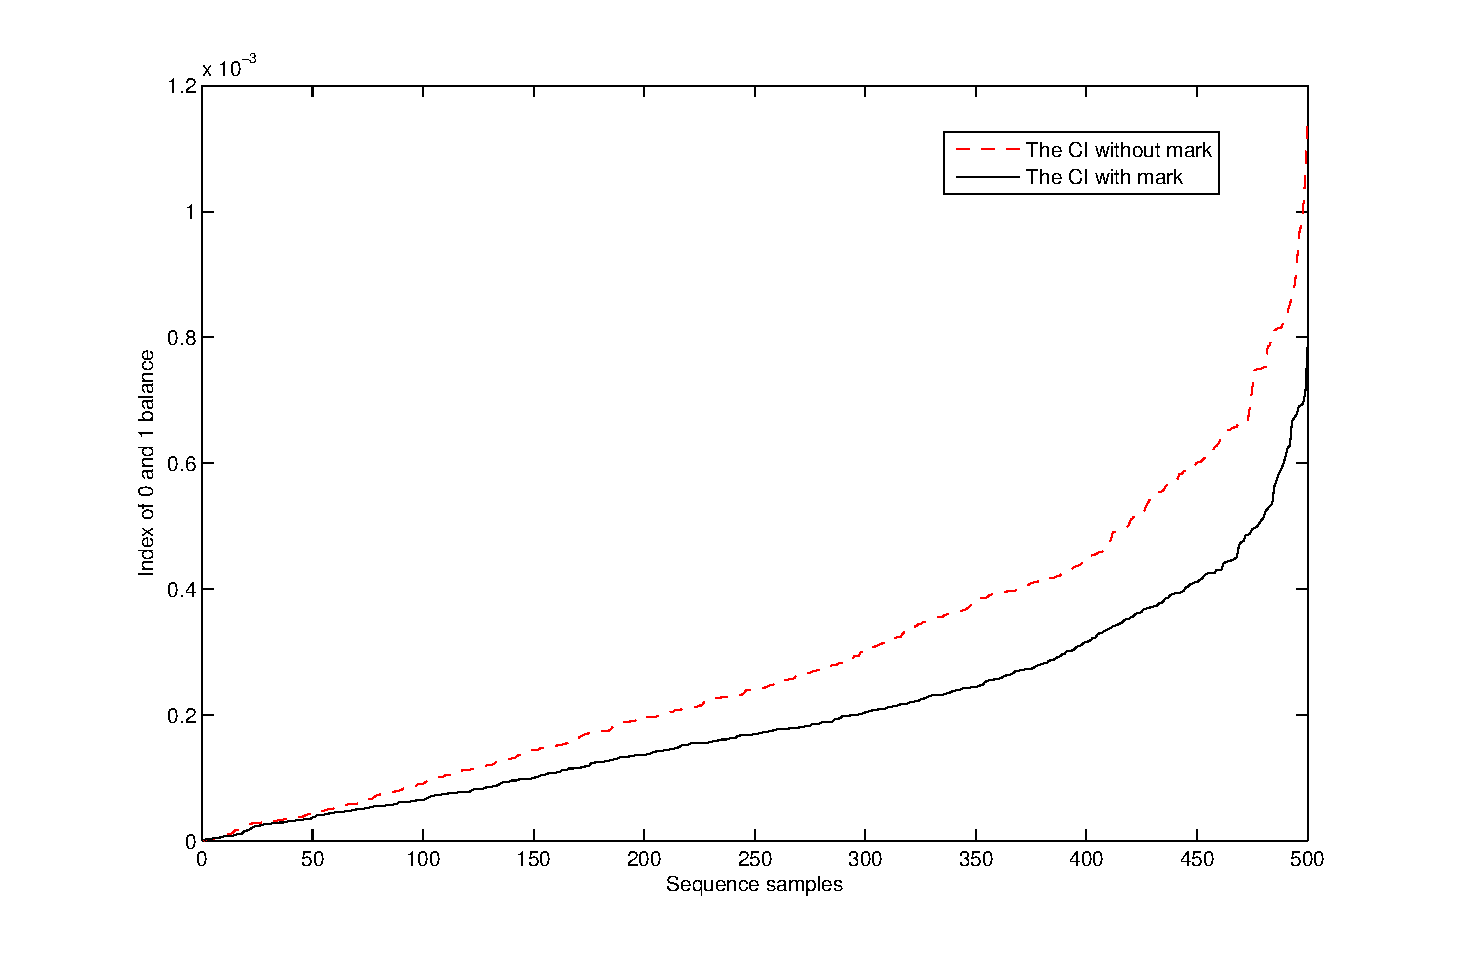
\includegraphics[width=3.85in]{nmark.eps}
\DeclareGraphicsExtensions.
\caption{Balance property}
\label{nmark}
\end{figure}


\subsection{CIPRNG version 2: the algorithm}

The basic design procedure of the novel generator is summed up in Algo.\ref{Chaotic iteration1}.
The internal state is $x$, the output state is $r$. $a$ and $b$ are those computed by the two input
PRNGs. The value $g_1(a)$ is an integer, defined as in Eq.(\ref{v2_g1}). Lastly, $\mathsf{N}$ is a constant 
defined by the user.
\begin{algorithm}
\textbf{Input:} the internal state $x$ ($\mathsf{N}$ bits)\\
\textbf{Output:} a state $r$ of $\mathsf{N}$ bits
\begin{algorithmic}[1]
\FOR{$i=0,\dots,N$}
{
\STATE$d_i\leftarrow{0}$\;
}
\ENDFOR
\STATE$a\leftarrow{PRNG1()}$\;
\STATE$m\leftarrow{f(a)}$\;
\STATE$k\leftarrow{m}$\;
\WHILE{$i=0,\dots,k$}

\STATE$b\leftarrow{PRNG2()~mod~\mathsf{N}}$\;
\STATE$S\leftarrow{b}$\;
    \IF{$d_S=0$}
    {
\STATE      $x_S\leftarrow{ \overline{x_S}}$\;
\STATE      $d_S\leftarrow{1}$\;
    
    }
    \ELSIF{$d_S=1$}
    {
\STATE      $k\leftarrow{ k+1}$\;
    }\ENDIF
\ENDWHILE
$r\leftarrow{x}$\;
return $r$\;
\medskip
\caption{An arbitrary round of the CI generator Version 2}
\label{Chaotic iteration1}
\end{algorithmic}
\end{algorithm}

Compare to CI Version 1, this latter version provides better statistical performance and speed \cite{bfgw11:ij}.

%As a comparison, the basic design procedure of the old generator 
%is recalled in Algorithm~\ref{Chaotic iteration2} ($a$ and $b$ are computed by two input PRNGs, 
%$\mathsf{N}$ and $c\geqslant 3\mathsf{N}$ are constants defined by the user). 
%See Subsection~\ref{Version 1 CI algorithms and examples} for further information.
%
%
%\begin{algorithm}
%\textbf{Input:} the internal state $x$ (an array of $\mathsf{N}$ 1-bit words)\\
%\textbf{Output:} an array $r$ of $\mathsf{N}$ 1-bit words
%\begin{algorithmic}[1]
%
%\STATE$a\leftarrow{PRNG1()}$;
%\STATE$m\leftarrow{a~mod~2+c}$;
%\WHILE{$i=0,\dots,m$}
%\STATE$b\leftarrow{PRNG2()}$;
%\STATE$S\leftarrow{b~mod~\mathsf{N}}$;
%\STATE$x_S\leftarrow{ \overline{x_S}}$;
%\ENDWHILE
%\STATE$r\leftarrow{x}$;
%\STATE return $r$;
%\medskip
%\caption{An arbitrary round of the old CI generator}
%\label{Chaotic iteration2}
%\end{algorithmic}
%\end{algorithm}
%

%\subsection{Illustrative Example of Version 2 CI (XORshift, XORshift)}
%
%In this example, $\mathsf{N} = 4$ is chosen for easy understanding and the input PRNG is XORshift PRNG. As stated before, the initial state of the system $x^0$ can be seeded by the decimal part $t$ of the current time. For example, if the current time in seconds since the Epoch is 1237632934.484088,
%so $t = 484088$, then $x^0 = t \text{ ($mod$ 16)}$ in binary digits, \emph{i.e.}, $x^0 = ( 0, 1, 0, 0)$.
%
%To compute $m$ sequence, Eq.(\ref{v2_g1}) can be adapted to this example as follows:
%\begin{equation}
%\label{m1 fuction}
%m^n=g_1(y^n)=
%\left\{
%\begin{array}{llccccc}
%0 & \text{ if }&0 &\leqslant&\frac{y^n}{2^{32}}&<&\frac{1}{16},\\
%1 & \text{ if }&\frac{1}{16} &\leqslant&\frac{y^n}{2^{32}}&<&\frac{5}{16} ,\\
%2 & \text{ if }&\frac{5}{16} &\leqslant&\frac{y^n}{2^{32}}&<&\frac{11}{16},\\
%3 & \text{ if }&\frac{11}{16} &\leqslant&\frac{y^n}{2^{32}}&<&\frac{15}{16},\\
%4 & \text{ if }&\frac{15}{16} &\leqslant&\frac{y^n}{2^{32}}&<&1,\\
%\end{array}
%\right.
%\end{equation}
%
%\noindent where $y$ is generated by XORshift seeded with the current time. 
%We can see that the probabilities of occurrences of $m=0$, $m=1$, $m=2$, $m=3$, $m=4$, 
%are $\frac{1}{16}$, $\frac{4}{16}$, $\frac{6}{16}$, $\frac{4}{16}$, $\frac{1}{16}$, respectively. 
%This $m$ determines what will be the next output $x$. For instance,
%\begin{itemize}
%\item If $m=0$, the following $x$ will be $( 0, 1, 0, 0)$.
%\item If $m=1$, the following $x$ can be $( 1, 1, 0, 0)$, $( 0, 0, 0, 0)$, $( 0, 1, 1, 0)$, or $( 0, 1, 0, 1)$.
%\item If $m=2$, the following $x$ can be $( 1, 0, 0, 0)$, $( 1, 1, 1, 0)$, $( 1, 1, 0, 1)$, $( 0, 0, 1, 0)$, $( 0, 0, 0, 1)$, or $( 0, 1, 1, 1)$.
%\item If $m=3$, the following $x$ can be $( 0, 0, 1, 1)$, $( 1, 1, 1, 1)$, $( 1, 0, 0, 1)$, or $( 1, 0, 1, 0)$.
%\item If $m=4$, the following $x$ will be $( 1, 0, 1, 1)$.
%\end{itemize}
%
%In this simulation, $m = 0, 4, 2, 2, 3, 4, 1, 1, 2, 3, 0, 1, 4,...$ Additionally, 
%$b$ is computed with a XORshift generator too, but with another seed. We have found 
%$b = 1, 4, 2, 2, 3, 3, 4, 1, 1, 4, 3, 2, 1,...$
%
%Chaotic iterations are made with initial state $x^0$, vectorial logical negation $f_0$, and
%strategy $S$. The result is presented in Tab.\ref{table application example}. Let us 
%recall that sequence $m$ gives the states $x^n$ to return, which are here $x^0, x^{0+4}, 
%x^{0+4+2}, \hdots$ So, in this example, the output of the generator is: 10100111101111110011... or 4,4,11,8,1...
%
%\begin{table*}[!t]
%%\renewcommand{\arraystretch}{1.3}
%\centering
%\begin{tabular}{|c|c@{}c|c@{}c@{}c@{}c@{}c@{}c|c@{}c@{}c|c@{}c@{}c@{}c|}
%\hline
%$m$ &0 & &4 & & & & & &2& &&2&&  &  \\ \hline
%$k$ &0 & &4 & & &$+1$ & & &2& &&2&$+1$&  &  \\ \hline
%$b$  &  & &1 &4&2&\underline{2}       &3& &3&4&&1&\underline{1}      &4&\\ \hline
%$d$  &r  & &r~$\left(\begin{array}{c}1\\0\\0\\0\end{array}\right)$ & $\left(\begin{array}{c}1\\0\\0\\1\end{array}\right)$ & $\left(\begin{array}{c}1\\1\\0\\1\end{array}\right)$ & & $\left(\begin{array}{c}1\\1\\1\\1\end{array}\right)$ && r~$\left(\begin{array}{c}0\\0\\1\\0\end{array}\right)$ &$\left(\begin{array}{c}0\\0\\1\\1\end{array}\right)$ &&r~$\left(\begin{array}{c}1\\0\\0\\0\end{array}\right)$ & &$\left(\begin{array}{c}1\\0\\0\\1\end{array}\right)$  &  \\ \hline
%$S$  &  & &1 &4&2&        &3& &3&4&&1& &4 &  \\ \hline
%$x^{0}$ &  &$x^{0}$ & & &  
%&  & &$x^{4}$ & & &   
%$x^{6}$& & &&$x^{8}$  \\
%%1ere ligne
%0 & &0 &$\xrightarrow{1} 1$ & &
% & &   &1   & & &
%1 &$\xrightarrow{1} 0$ & & & 0\\
%%2eme ligne
%1 &  &1 &   &   &
%$\xrightarrow{2} 0$ & & &0 & & &
%0 & &  &&0\\
%%3eme ligne
%0 & &0 & & &
% & &$\xrightarrow{3} 1$ &1 &$\xrightarrow{3} 0$ & &
%0 &   & & &0  \\
%% 4eme ligne
%0 & &0  & &$\xrightarrow{4} 1$ &
% & & &1 & &$\xrightarrow{4} 0$ &
%0 & & &$\xrightarrow{4} 1$&1 \\
%\hline
%\end{tabular}\\
%\vspace{0.5cm}
%Binary Output: $x_1^{0}x_2^{0}x_3^{0}x_4^{0}x_1^{4}x_2^{4}x_3^{4}x_4^{4}x_1^{6}x_2^{6}... = 0100101110000001...$\\
%Integer Output:
%$x^{0},x^{4},x^{6},x^{8}... = 4,11,8,1...$
%\caption{Example of Version 2 CI(XORshift,XORshift) generation}
%\label{table application example}
%\end{table*}
